\documentclass{../tuda-exercise}

% Title information
\version{20. November 2021}
\sheetnumber{8}

% Fix url underfull hbox
\Urlmuskip=0mu plus 10mu

\begin{document}

  \maketitle

  \begin{task}[credit=\stars{0}{3}]{Theoriefragen}
    \begin{enumerate}
      \item Welche Vorteile ergeben sich durch die Nutzung von Generics?
      \item Diskutieren Sie Vor- und Nachteile von Collections gegenüber Arrays unter den
      folgenden Aspekten:
      \begin{enumerate}
        [label=(\alph*)]
        \item Finden von Elementen
        \item Einfügen neuer Elemente
        \item Löschen von Elementen
      \end{enumerate}
      \item Auch in Racket haben Sie Listen kennengelernt. Ist das Java-Interface
      \item \href{https://docs.oracle.com/en/java/javase/11/docs/api/java.base/java/util/List.html}
      {\inlinejava{java.util.List}} vergleichbar mit den Listen aus Racket?
    \end{enumerate}

    \begin{solution}
      \begin{enumerate}
        \item Die Verwendung von Generics ermöglicht es weniger redundanten Code zu schreiben, da
        man eine Klasse/Methode durch Generizität auf mehrere Referenztypen anwenden kann, ohne
        diese immer wieder neu speziell für einen Typ schreiben zu müssen. Ein Beispiel dafür ist
        das Interface
        \item \href{https://docs.oracle.com/en/java/javase/11/docs/api/java.base/java/util/Collection.html}
        {\inlinejava{java.util.Collection}} in Java.
        \item
        \begin{enumerate}
          [label=(\alph*)]
          \item Ein Array bietet zwei Möglichkeiten nach Elementen zu suchen:
          \begin{enumerate}
            \item Indexsuche: Auf das Element kann via Index direkt zugegriffen werden.
            \item Elementsuche: Das Array kann mittels einer Schleife durchlaufen werden.
          \end{enumerate}
          In einer Collection hingegen kann das Element nur via Elementensuche gefunden werden.
          \item Arrays haben keine dynamische Größe, weshalb nur erschwert Elemente eingefügt
          werden können, wenn das Array schon voll ist. Das kann man bspw. mit der Erstellung
          eines neuen größeren Arrays und kopieren der Elemente vom Alten ins Neue umgehen.
          Collections hingegen haben eine variable Größe, d.h. man kann ohne große Bedenken immer
          neue Elemente einfügen.
          \item Das Löschen von Elementen in einem Array ist nicht möglich. Sie können bspw. nur
          durch den Wert \inlinejava{null} überschrieben werden. In einer \inlinejava{java.util
          .Collection} können Elemente gelöscht werden mittels bspw. \inlinejava{boolean}
          \inlinejava{remove(Object o)}.
        \end{enumerate}
        \item Das Java-Interface
        \href{https://docs.oracle.com/en/java/javase/11/docs/api/java.base/java/util/List.html}
        {\inlinejava{java.util.List}} ist nicht mit den Listen aus Racket vergleichbar, da Listen
        in Racket nicht dynamisch sind. In Java sind Listen von der Größe her deutlich flexibler
        als in Racket. Ein weiterer Unterschied zwischen \inlinejava{java.util.List} und Listen
        aus Racket ist, dass die Liste in Racket beliebige Typen enthalten kann. In
        \inlinejava{java.util.List} können nur Elemente von einem festen Typ gespeichert werden.
        Der statische Typ bestimmt, welche Typen die Elemente in der Liste haben müssen und der
        dynamische Typ kann entweder gleich oder eine abgeleitete Klasse vom statischen Typ sein.
      \end{enumerate}
    \end{solution}
  \end{task}


  \begin{task}[credit=\stars{1}{3}]{Collections und Exceptions}
    Gegeben sei folgender Codeausschnitt:

    \lstinputlisting[style=Java]{codes/V2_Task.java}

    \begin{enumerate}
      [label=(\arabic*)]
      \item Beschreiben Sie kurz und bündig, aber präzise und unmissverständlich was der oben
      gegebene Code macht.
    \end{enumerate}

    \begin{enumerate}
      [label=(2.\arabic*)]
      \item An welcher Stelle kann im Code eine Exception geworfen werden? Durch welche Eingaben
      wird sie ausgelöst?
      \item Modifizieren Sie den Code mithilfe eines
      \inlinejava{try}/\inlinejava{catch}-Blockes so, dass in diesen
      Fällen die Nachricht der Exception auf der Konsole ausgegeben wird.
    \end{enumerate}

    \begin{solution}
      \begin{enumerate}
        [label=(\arabic*)]
        \item Die Methode \inlinejava{foo} liefert die größte ungerade Zahl im Array zurück, die
        kleiner oder gleich \inlinejava{n} und größer als \(0\) ist.
      \end{enumerate}

      \begin{enumerate}
        [label=(2.\arabic*)]
        \item
        \begin{itemize}
          \item Zeile 3: Wenn das übergebene Array gleich \inlinejava{null} ist, so wird eine
          \inlinejava{NullPointerException} geworfen.
          \item Zeile 8: Falls das Array keine ungerade Zahl kleiner oder gleich \inlinejava{n}
          enthält, so wirft der Aufruf von
          \href{https://docs.oracle.com/en/java/javase/11/docs/api/java.base/java/util/LinkedList.html#getLast()}
          {\inlinejava{getLast()}} eine \inlinejava{NoSuchElementException}.
        \end{itemize}
        \item\hfill
        \lstinputlisting[style=Java]{codes/V2_Solution.java}
      \end{enumerate}
    \end{solution}
  \end{task}

  \clearpage

  \begin{task}[credit=\stars{1}{3}]{A-well-a bird bird bird, bird is the word Part I}
    \label{task:V3}
    In dieser Aufgabe betrachten wir eine stark reduzierte Typhierarchie zur Modellierung von
    Vögeln. Dabei stellen die Pfeile die Erbbeziehungen zwischen Klassen dar. Dazu ist das
    folgende Typdiagramm in Abbildung \ref{figure:V3} gegeben. Hier ist \inlinejava{Bird} also
    die Oberklasse und die drei anderen Klassen sind Erben dieser.

    \begin{figure}[h]
      \centering
      \begin{tikzpicture}[
        every node/.style={
        draw,
        line width=1pt,
        minimum height=30pt,
        minimum width=50pt,
        transform shape,
        shape=rectangle,
        },
        arrow/.style={-stealth}
      ]
        \node (t) {Bird};
        \node[below= of {t}] (c) {Ostrich};
        \node[left= of {c}] (l) {Penguin};
        \node[right= of {c}] (r) {Dodo};

        \draw[arrow] (c) -- (t);
        \draw [-] (l) |- ($(c)!0.5!(t)$);
        \draw [-] (r) |- ($(c)!0.5!(t)$);
      \end{tikzpicture}
      \caption{Typhierarchie mit drei Vogelarten}
      \label{figure:V3}
    \end{figure}

    Wir nutzen die generische Datenstruktur \inlinejava{Vector<E>}. Dabei beschränken wir uns auf
    die Methode \inlinejava{void add(E entry)}, die ein Element vom Typ \inlinejava{E} in den
    Vector einfügt.

    \begin{enumerate}
      [label=(\arabic*):]
      \item Deklarieren und initialisieren Sie eine Variable \inlinejava{v} mit dem
      \textbf{statischen} Basistyp \inlinejava{List} und dem \textbf{dynamischen} Typ
      \inlinejava{Vector}, so dass darin genau Objekte der Typen \inlinejava{Birds},
      \inlinejava{Penguin}, \inlinejava{Ostrich} und \inlinejava{Dodo} gespeichert werden können.
      Nutzen Sie generische Typparameter!
      \item Geben Sie Java-Code an, um in den obigen \inlinejava{Vector v} jeweils ein neues
      Element vom Typ \inlinejava{Penguin} und \inlinejava{Ostrich} einzufügen. Sie dürfen zur
      Vereinfachung die Parameter der Konstruktoren der Klassen \inlinejava{Penguin} und
      \inlinejava{Ostrich} durch ..... abkürzen.
      \item Die Methode \inlinejava{addAll(Birds)} existiert im Interface \inlinejava{List} und
      fügt eine gesamte \inlinejava{Collection} in eine gegebene \inlinejava{Collection} ein. Die
      Klasse \inlinejava{ArrayList} implementiert das Interface \inlinejava{List}. Ist die
      folgende Anweisung – nachdem Code der vorherigen Aufgaben – dann zulässig?
      \lstinputlisting[style=Java]{codes/V3_Task.java}
    \end{enumerate}

    \begin{solution}
      \begin{enumerate}
        [label=(\arabic*):]
        \item\hfill
        \lstinputlisting[style=Java]{codes/V3_01_Solution.java}
        \item\hfill
        \lstinputlisting[style=Java]{codes/V3_02_Solution.java}
        \item Die Anweisung ist nicht zulässig, da
        \href{https://docs.oracle.com/en/java/javase/11/docs/api/java.base/java/util/Collection.html#addAll(java.util.Collection)}
        {\inlinejava{addAll}} eine \inlinejava{Collection<? extends Dodo>} erwartet, d.h. nur
        eine Liste von \inlinejava{Dodo} (Typparameter) oder Klassen, die von \inlinejava{Dodo}
        abgeleitet sind. Jedoch ist \inlinejava{v} eine Liste von Vögeln (\inlinejava{Bird}).
      \end{enumerate}
    \end{solution}
  \end{task}

  \begin{task}[credit=\stars{1}{3}]{Elemente tauschen}
    Schreiben Sie eine Methode

    \begin{center}
      \inlinejava{void switchElements(T[] a, int i, int j) throws IllegalArgumentException}
    \end{center}

    Die Methode vertauscht die Elemente im übergebenen Array \inlinejava{a} an den zwei
    angegebenen Indizes \inlinejava{i} und \inlinejava{j}. Falls für \inlinejava{a} eine
    \inlinejava{null}-Referenz übergeben wird oder einer der Indizes nicht in dem Array liegt,
    soll eine \inlinejava{IllegalArgumentException} geworfen werden.

    \begin{solution}
      \lstinputlisting[style=Java]{codes/V4_Solution.java}
    \end{solution}
  \end{task}

  \clearpage

  \begin{task}[credit=\stars{2}{3}]{Typhierarchie}
    \begin{minipage}{0.7\textwidth}
      Wir betrachten eine Typhierarchie (dargestellt in der Abbildung rechts) mit einer Klasse
      \inlinejava{A} und einem Erben \inlinejava{B}. Von \inlinejava{B} ist wiederum
      \inlinejava{C} abgeleitet. Markieren Sie im folgenden Java-Code jeweils hinter
      \inlinejava{//}, ob der Compiler die Zeile akzeptiert (\enquote{Okay}) der ablehnt
      (\enquote{Fehler}). Lösen Sie die Aufgabe zunächst durch eigene Überlegungen und überprüfen
      Sie erst später mittels Eclipse.
    \end{minipage}
    \hfill
    \begin{minipage}{0.2\textwidth}
      \begin{tikzpicture}[
        every node/.style={
        draw,
        line width=1pt,
        minimum height=20pt,
        minimum width=40pt,
        node distance=15pt,
        transform shape,
        shape=rectangle,
        }
      ]
        \node (a) {A};
        \node[below=of {a}] (b) {B};
        \node[below=of {b}] (c) {C};
        \draw[-stealth] (b) -- (a);
        \draw[-stealth] (c) -- (b);
      \end{tikzpicture}
    \end{minipage}

    \lstinputlisting[style=Java]{codes/V5_Task.java}

    \clearpagesolution

    \begin{solution}
      \lstinputlisting[style=Java]{codes/V5_Solution.java}

      \begin{note}[title=Information:]
        Eine Wildcard ist ein spezieller Typparameter für die Instanziierung von generischen
        (parametrisierten) Typen und wird mit einem \inlinejava{?} gekennzeichnet. Sie wird für
        die Einschränkung bei dieser Instanziierung verwendet, was eine Flexibilität von
        Typparametern bei Objekten ermöglicht. Dabei unterscheiden wir zwei Arten von Wildcards.
        Einmal können die Parameter nach oben durch \inlinejava{extends} beschränkt werden und
        einmal nach unten durch die Verwendung von \inlinejava{super}:

        \begin{itemize}
          \item Beschränkung der Parameter nach oben
          \\
          Bei der Upper bounded Wildcard ist der Typparameter nach oben in der
          Vererbungshierachie beschränkt. Das ermöglicht es aktuale Parameter zu verwenden, die
          anstelle von \inlinejava{T} mit einer von \inlinejava{T} abgeleiteten Klassen
          instanziiert sind.

          \br

          Dadurch wird außerdem das Lesen vom Typ \inlinejava{T} (\inlinejava{T} ist ein
          Platzhalter für einen konkreten Typ) erlaubt, welcher im Wildcard spezifiziert wurde
          und das Einfügen von \inlinejava{null}. Das Einfügen von anderen Typen ist nicht
          zulässig, da die Typsicherheit nicht garantiert werden kann. Als Veranschaulichung
          nehmen wir folgendes Beispiel:

          \begin{center}
            List<? extends Number>
          \end{center}

          Wir wissen, dass der Typparameter der Liste entweder
          \href{https://docs.oracle.com/en/java/javase/11/docs/api/java.base/java/lang/Number.html}{\inlinejava{Number}}
          selbst oder ein Subtyp davon ist, aber nicht genau welcher konkrete Typ es ist. Wir
          wollen nun einen \inlinejava{Double}-Wert hinzufügen, da \inlinejava{Double} eine
          Subklasse von \inlinejava{Number} ist. Aber das zu tun wäre nicht typsicher, da der
          tatsächliche Typparameter der Liste nicht unbedingt \inlinejava{Double} sein muss,
          sondern auch ein anderer Subtyp oder \inlinejava{Number} selbst sein kann.
          Beispielsweise könnten, falls die Liste in Wahrheit eine Liste von \inlinejava{Integer}
          (\inlinejava{ArrayList<Integer>}) ist, keine \inlinejava{Double}-Werte in der Liste
          gespeichert werden.

          \item Beschränkung der Parameter nach unten
          \\
          Bei einer Lower bounded Wildcard ist der Typparameter nach unten in der
          Vererbungshierachie beschränkt. Das ermöglicht es anstelle von \inlinejava{T} eine der
          von \inlinejava{T} direkt oder indirekte Basisklasse, sowie alle von \inlinejava{T}
          implementierten Interfaces, als aktuale Parameter zu verwenden.

          \br

          Dadurch wird außerdem beim Schreiben die Verwendung von \inlinejava{T} selbst oder von
          dessen Subtyp erlaubt. Das liegt daran, dass \inlinejava{T} oder ein Subtyp von
          \inlinejava{T} auch indirekt vom Typ deren gemeinsamer Superklasse. Beispielsweise ist
          \href{https://docs.oracle.com/en/java/javase/11/docs/api/java.base/java/lang/Integer.html}
          {\inlinejava{Integer}} indirekt auch eine
          \href{https://docs.oracle.com/en/java/javase/11/docs/api/java.base/java/lang/Number.html}
          {\inlinejava{Number}}, da
          \href{https://docs.oracle.com/en/java/javase/11/docs/api/java.base/java/lang/Integer.html}
          {\inlinejava{Integer}} ein Subtyp von
          \href{https://docs.oracle.com/en/java/javase/11/docs/api/java.base/java/lang/Number.html}
          {\inlinejava{Number}} ist. Beim Lesen ist nur das Lesen von \inlinejava{Object}
          garantiert, da es Superklasse von allen Klassen ist. Wir können diese Tatsache an dem
          folgendes Beispiel veraschaulichen:

          \begin{center}
            List<? super Number>
          \end{center}

          Wir wissen, dass der Typparameter der Liste entweder \inlinejava{Number} oder ein
          Supertyp davon ist. Das heißt es sind folgende Typen möglich:

          \begin{itemize}
            \item \href{https://docs.oracle.com/en/java/javase/11/docs/api/java.base/java/lang/Number.html}
            {\inlinejava{Number}}
            \item \href{https://docs.oracle.com/en/java/javase/11/docs/api/java.base/java/io/Serializable.html}
            {\inlinejava{Serializable}}
            \item \href{https://docs.oracle.com/en/java/javase/11/docs/api/java.base/java/lang/Object.html}
            {\inlinejava{Object}}
          \end{itemize}

          In allen Fällen können wir eine \inlinejava{Number} oder einen Subtyp davon einfügen.
          Wenn wir aber eine \inlinejava{Number} lesen möchten, wäre dies nicht typsicher, da der
          tatsächliche Typparameter der Liste nicht unbedingt \inlinejava{Number} sein muss,
          sondern auch ein Supertyp von \inlinejava{Number} sein kann. Deshalb würde
          beispielsweise, falls die Liste in Wahrheit eine Liste von \inlinejava{Object}
          (\inlinejava{ArrayList<Object>}) ist, ein Element dessen nicht zwangsweise eine
          \inlinejava{Number} sein.
        \end{itemize}
      \end{note}
    \end{solution}
  \end{task}

  \clearpage

  \begin{task}[credit=\stars{2}{3}]{A-well-a bird bird bird, bird is the word Part II}
    Wir erweitern unsere Typhierarchie für Vögel aus Aufgabe \hyperref{task:V3}{V3} und
    betrachten neben den nicht-fliegen den Vögeln nun auch ihre flatternden Artgenossen.

    \begin{figure}[h]
      \centering
      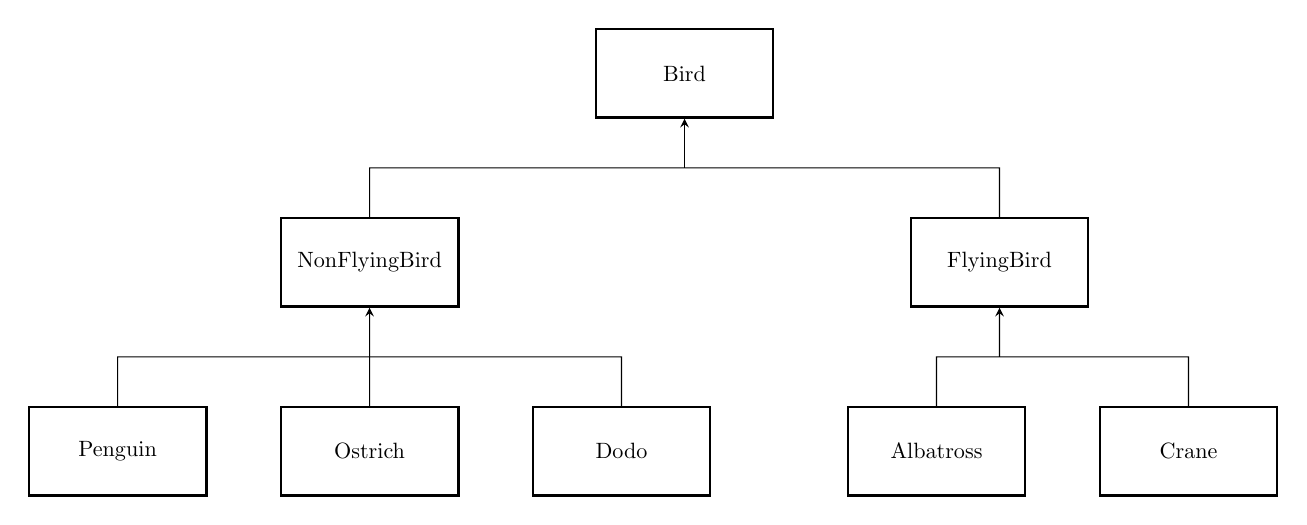
\begin{tikzpicture}[
        every node/.style={
        draw,
        line width=1pt,
        minimum height=40pt,
        minimum width=80pt,
        transform shape,
        shape=rectangle,
        },
        scale=.8,
        transform shape
      ]
        \node (a) at (0, 0) {Bird};
        \node (b) at (-5, -3) {NonFlyingBird};
        \node (c) at (5, -3) {FlyingBird};
        \node (d) at (-9, -6) {Penguin};
        \node (e) at (-5, -6) {Ostrich};
        \node (g) at (-1, -6) {Dodo};
        \node (h) at (4, -6) {Albatross};
        \node (i) at (8, -6) {Crane};

        \draw[-stealth] (0, -1.5) -- (a);
        \draw (b.north) -- (-5, -1.5) -- (0, -1.5);
        \draw (c.north) -- (5, -1.5) -- (0, -1.5);

        \draw[-stealth] (e) -- (b);
        \draw (d.north) -- (-9, -4.5) -- (-5, -4.5);
        \draw (g.north) -- (-1, -4.5) -- (-5, -4.5);

        \draw[-stealth] (5, -4.5) -- (c);
        \draw (h.north) -- (4, -4.5) -- (5, -4.5);
        \draw (i.north) -- (8, -4.5) -- (5, -4.5);
      \end{tikzpicture}
      \caption{Erweiterte Typhierarchie}
    \end{figure}

    Vervollständigen Sie die untenstehenden Deklarationen der Methoden. Dabei sind nur die mit
    ..... markierten Stellen zu bearbeiten! Geben Sie zu jeder Typangabe eine kurze Erklärung,
    warum genau diese Typangabe die am besten passende oder korrekte ist.
    \\
    \textit{Ihre Lösungen sollen möglichst weitgehend die Typsicherheit garantieren, aber
    gleichzeitig flexibel für möglichst viele konkrete Parametertypen sein.}

    \br

    Es sind immer generische \textbf{Sub}typen zu nutzen.

    \begin{note}[title=Hinweis:, color=tuda-orange]
      Zur Vereinfachung wird in den Beispielen nicht auf \inlinejava{null} oder auf eine leere
      Liste getestet.
    \end{note}

    \begin{enumerate}
      [label=(\arabic*):]
      \item Die Methode \inlinejava{getFirst(List<.....> aListOfBirds)} liefert den ersten Vogel
      einer (nicht-leeren) Liste. Das Ergebnis muss kompatibel zum Typ \inlinejava{Bird} sein.
      \lstinputlisting[style=Java]{codes/V6_01_Task.java}
      \item Die Methode \inlinejava{void add(Birds b, List<.....> aListOfBirds)} fügt einen neuen
      Vogel in die Liste ein. Es sollen dabei Vögel jedes bekannten Typs eingefügt werden können.

      \lstinputlisting[style=Java]{codes/V6_02_Task.java}
    \end{enumerate}

    \clearpagesolution

    \begin{solution}
      \begin{enumerate}
        [label=(\arabic*):]
        \item Laut Aufgabenstellung muss die Liste beliebige Vögel enthalten können und ohne
        Typecast immer \inlinejava{Birds} liefern. Prinzipiell könnte man hier zwar auch
        \inlinejava{List<Bird>} nutzen, aber dies schränkt die Menge der möglichen konkreten
        Typen der als Parameter übergebenen Listen ein und ist daher schlechter. Die
        Beschränkungen von \inlinejava{List<? extends Birds>} – kein Einfügen von Elementen
        möglich außer null – sind hier irrelevant.

        \lstinputlisting[style=Java]{codes/V6_01_Solution.java}

        \item \inlinejava{List<? extends Birds>} und \inlinejava{List<?>} erlauben kein Einfügen
        von Werten außer \inlinejava{null}. Der Typ \inlinejava{List<Birds>} wäre zu unflexibel,
        da dabei die Menge der möglichen konkreten Typen der als Parameter übergebenen Listen
        eingeschränkt wird.

        \lstinputlisting[style=Java]{codes/V6_02_Solution.java}
      \end{enumerate}
    \end{solution}
  \end{task}

  \clearpage

  \begin{task}[credit=\stars{2}{3}]{Array Utility-Klasse}
    In dieser Aufgabe wollen wir eine bereits vorhandene Utility-Klasse, für Arrays vom Datentyp
    \inlinejava{int}, so umschreiben, dass diese für jeden beliebigen Datentyp verwendet werden
    kann. Die Klasse \inlinejava{ArrayUtils} implementiert folgende Methoden:

    \br

    \inlinejava{void printArray (int[] array)} bekommt ein \inlinejava{int}-Array übergeben und
    gibt dessen Elemente auf der Konsole aus.

    \lstinputlisting[style=Java]{codes/V7_01_Task.java}

    \inlinejava{int getArrayIndex(int[] array, int value)} bekommt ein \inlinejava{int}-Array und
    einen Wert übergeben und durchsucht das Array nach dem übergebenen Wert. Wird der Wert
    gefunden, wird dessen Index im Array zurückgegeben, andernfalls \inlinejava{-1}.

    \lstinputlisting[style=Java]{codes/V7_02_Task.java}

    \inlinejava{void simpleSort(int[] array)} sortiert das übergebene \inlinejava{int}-Array in
    aufsteigender
    Reihenfolge.

    \lstinputlisting[style=Java]{codes/V7_03_Task.java}

    \clearpage

    Schreiben Sie nun eine Klasse \inlinejava{GenericArrayUtils}, die alle drei oben genannten
    Methoden mit einem beliebigen Datentyp \inlinejava{T}, bzw. \inlinejava{T[]} für Arrays,
    implementiert.

    \begin{note}[title=Hinweis:, color=tuda-orange]
      Überlegen Sie sich, wie Sie Elemente vom Typ \inlinejava{T} miteinander vergleichen können
      und welche Voraussetzung dieser Typ \inlinejava{T} mit sich bringen muss. Wie kann sich das
      im Klassenkopf der zu implementierenden Klasse widerspiegeln?
    \end{note}

    \begin{solution}
      \lstinputlisting[style=Java, lastline=37]{codes/V7_Solution.java}

      \clearpage

      \lstinputlisting[style=Java, firstline=38, firstnumber=38]{codes/V7_Solution.java}
    \end{solution}
  \end{task}

  \clearpagesolution

  \begin{task}[credit=\stars{3}{3}]{XYZ}
    Gegeben seien die folgenden Klassen:

    \lstinputlisting[style=Java]{codes/V8_Task.java}

    Erweitern Sie nun die Klasse \inlinejava{Utils} um eine \inlinejava{public}-Klassenmethode
    \inlinejava{intoMap}, ohne dabei den Klassenkopf zu modifizieren. Die Methode bekommt eine
    \inlinejava{java.util.List} von Tripeln übergeben und gibt eine \inlinejava{java.util.Map}
    zurück. Jedes \inlinejava{Triple} in der Liste wird in die \inlinejava{Map} überführt, indem
    Sie die \inlinejava{x}-Variable des Triples als Schlüssel verwenden und ein neues Paar aus
    der \inlinejava{y}- und \inlinejava{z}-Variable des Triples erstellen, um dies als Wert des
    zugehörigen Schlüssels zu verwenden.

    \begin{solution}
      \lstinputlisting[style=Java]{codes/V8_Solution.java}
    \end{solution}
  \end{task}

  \clearpage

  \begin{task}[credit=\stars{3}{3}]{Matrizenmultiplikation}
    In dieser Aufgabe wollen wir eine Matrix Klasse implementieren, die es uns erlaubt jeden
    beliebigen vergleichbaren Datentyp unter Anwendung von Java Generics mit ihr zu verwenden.

    \br

    Um Ihnen die Aufgabe zu erleichtern, wird ihnen ein Interface bereitgestellt, welches benutzt
    werden soll um arithmetische Operationen mit den Matrizen durchzuführen. Bevor man einen
    Datentyp mit unserer \inlinejava{Matrix} Klasse benutzen kann, muss man zuvor das
    arithmetische Interface für diesen konkreten Datentyp implementieren. Machen Sie sich mit den
    Beispielen auf der folgenden Seite vertraut.

    \br

    \textbf{Generisches Interface:}

    \lstinputlisting[style=Java]{codes/V9_01_Task.java}

    \clearpage

    \textbf{Konkrete Implementierung für Gleitkommazahlen mit dem Datentyp Float:}

    \lstinputlisting[style=Java]{codes/V9_02_Task.java}

    Bearbeiten Sie ausgehend davon die Aufgaben auf der nächsten Seite.

    \begin{subtask*}{Erstellen der Matrix-Klasse}
      Erstellen Sie zunächst die Klasse \inlinejava{public class Matrix<T extends Comparable<T>>},
      ie die folgenden aufgezählten Variablen besitzt:

      \begin{itemize}
        \item \inlinejava{private Arithmetic<T> arithmetic} ist zuständig für das Durchführen von
        arithmetischen Operationen.
        \item \inlinejava{private LinkedList<LinkedList<T>> data} enthält die Daten der Matrix.
        Hierbei repräsentiert die äußere \inlinejava{LinkedList} die Reihen und die innere
        \inlinejava{LinkedList} die Spalten der Matrix.
        \item \inlinejava{private int rows} wird zum speichern der aktuellen Anzahl der Reihen
        der Matrix verwendet.
        \item \inlinejava{private int columns} wird zum speichern der aktuellen Anzahl der
        Spalten der Matrix verwendet.
      \end{itemize}

      Implementieren Sie nun folgende Methoden:

      \begin{itemize}
        \item \inlinejava{public Matrix(int rows, int columns, Arithmetic<T> arithmetic)} erhält
        die gewünschte Größe der Matrix in Form von Reihen und Spalten und ein entsprechendes
        Objekt dessen Klasse das arithmetische Interface implementiert. Alle übergebenen
        Variablen dieser Methode sollen in den entsprechenden Objektvariablen gespeichert werden.
        Zusätzlich soll jeder Zellenwert mit \inlinejava{arithmetic.zero()} initialisiert werden.
        \item \inlinejava{public int getRows()} gibt die aktuelle Anzahl der Reihen der Matrix
        zurück.
        \item \inlinejava{public int getColumns()} gibt die aktuelle Anzahl der Spalten der
        Matrix zurück.
        \item \inlinejava{public T getCell(int row, int column)} erhält den Index einer Reihe
        sowie den Index einer Spalte und gibt den Wert der Zelle zurück.
        \item \inlinejava{public void setCell(int row, int column, T value)} erhält den Index
        einer Reihe sowie den Index einer Spalte und einen gewünschten Wert und setzt diesen an
        der entsprechenden Stelle in der Matrix ein.
      \end{itemize}

      \begin{solution}
        \lstinputlisting[style=Java, lastline=42]{codes/V9_1_Solution.java}

        \clearpage

        \lstinputlisting[style=Java, firstline=43, firstnumber=43]{codes/V9_1_Solution.java}
      \end{solution}
    \end{subtask*}

    \begin{subtask*}{Addition und Multiplikation}
      Implementieren\dots

      \br

      \dots Sie nun die Methode \inlinejava{public Matrix<T> add(Matrix<T> other)}. Diese erhält
      eine andere Matrix, addiert die übergebene Matrix und die Matrix, auf der die Methode
      aufgerufen wurde, miteinander und gibt das Ergebnis der Addition zurück. Sollten die
      Reihen- und/oder Spaltenanzahl der beiden Matrizen nicht übereinstimmen, soll
      \inlinejava{null} zurückgegeben werden.

      \br

      \dots Sie nun die Methode \inlinejava{public Matrix<T> mul(Matrix<T> other)}. Diese erhält
      eine andere Matrix, multipliziert die übergebene Matrix und die Matrix, auf der die Methode
      aufgerufen wurde, miteinander und gibt das Ergebnis der Multiplikation zurück. Sollten die
      Spaltenanzahl der aktuellen Matrix sich von der Reihenanzahl der übergebenen Matrix
      unterscheiden, soll \inlinejava{null} zurückgegeben werden.

      \clearpagesolution

      \begin{solution}
        \lstinputlisting[style=Java]{codes/V9_2_Solution.java}
      \end{solution}
    \end{subtask*}
  \end{task}
\end{document}
